\documentclass[aspectratio=169]{beamer}

% Language setup
\usepackage[magyar]{babel} % Babel for Hungarian
\usepackage[T1]{fontenc} % Output character encoding
\usepackage[utf8]{inputenc} % Input character encoding
\selectlanguage{magyar}

% Beamer styling setup
\usetheme{Boadilla}
\usecolortheme{default}
%\setbeamercolor{titlelike}{parent=structure,bg=gray!15}
\setbeamertemplate{navigation symbols}{}
\setbeamertemplate{caption}[numbered]
%

% Spacing setup
\setlength{\parindent}{0pt} % No paragraph indenting
\setlength{\parskip}{5pt} % Set spacing between paragraphs
\frenchspacing
\newcommand{\mkspace}{\vspace{19pt}}
\newcommand{\rmspace}{\vspace{-19pt}}
\newcommand{\emptyline}{\vspace{\baselineskip}}
%

% Dependency setup
\usepackage{tikz}
\usetikzlibrary{decorations.markings}
\usetikzlibrary{calc}
%

% Style setup
\usepackage{caption}
\usepackage{subcaption}
\captionsetup{format=plain, font=footnotesize, labelformat=empty}
%

% Notation setup
\usepackage{physics} % Braket notation

% Add qi.svg logo
\usepackage{svg}
\usepackage[absolute,overlay]{textpos}

% Newline in cell
\usepackage{makecell}

\author[Nemkin Viktória]{Nemkin Viktória}
\institute[]{
\begin{small}dr. Friedl Katalin\end{small}\\
\begin{footnotesize}Számítástudományi és Információelméleti Tanszék\end{footnotesize}
}
\title{Memóriafelhasználás optimalizálása}
\subtitle{kvantumalgoritmusok szimulációja során}
\date{}

\begin{document}

\begin{frame}
\titlepage

\begin{textblock*}{150pt}(280pt,200pt) % {block width} (coords)
\includesvg[inkscape=overwrite,width=150pt]{./figures/qi.svg}
\end{textblock*}
\end{frame}


\begin{frame}{Motiváció: Protein folding kvantuszámítógépen}

\begin{columns}
\begin{column}{0.5\textwidth}
\begin{itemize}
    \item Protein lánc beágyazása 3D rács pontjaiba.
    \item Orákulum: Egymás mellé kerülő csúcsok energiaviszonyának lepontozása.
    \item Grover keresés: Energiaminimum megtalálása.
    \item Operátorok: Hadmard, Grover, WeightedAdder, Multi-Controlled NOT.
\end{itemize}

\end{column}
\begin{column}{0.5\textwidth}
    \begin{center}
     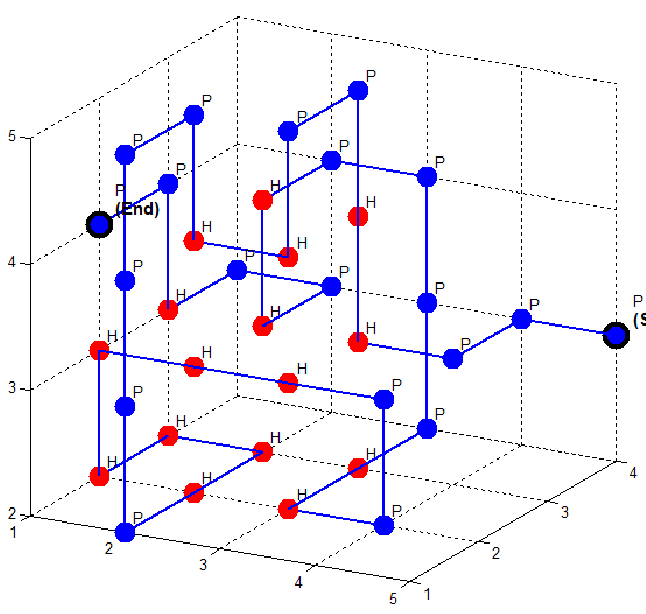
\includegraphics[width=\textwidth]{./figures/Protein-folds-with-length-36-amino-acids-18-contacts.png}
     \end{center}
\end{column}
\end{columns}

\end{frame}


\begin{frame}{Probléma: Memóriafelhasználás}
\begin{itemize}
    \item Operátorok exponenciálisan sok memóriát fogyasztanak.
\end{itemize}
\end{frame}

\end{document}